\documentclass[a4paper, fleqn, 10pt]{report}
\usepackage[utf8]{inputenc}
\usepackage{t1enc}
\usepackage[table, usenames,dvipsnames,svgnames]{xcolor}
\usepackage[pdftex]{graphicx}
\usepackage{booktabs}
\usepackage{setspace}
\onehalfspacing
\usepackage{fullpage}
\usepackage{enumerate}
\usepackage{multicol}
\usepackage{tikz}
\usepackage{amsmath, amsthm, amssymb}
\usepackage{caption}
\usepackage{subcaption}
\usepackage{multirow}

\usepackage{newtxtext}
\usepackage[libertine]{newtxmath}
%\usepackage{fourier}


\theoremstyle{definition}
\newtheorem{prb}{Problem}[chapter]
\newenvironment{prb*}[1]
  {\renewcommand\theprb{\thechapter.\arabic{prb}\rlap{$^{#1}$}}\prb}
  {\endprb}
  

\newcommand{\R}{\mathbf{R}}
\newcommand{\N}{\mathbf{N}}
\newcommand{\Z}{\mathbf{Z}}
\newcommand{\Q}{\mathbf{Q}}
\newcommand{\C}{\mathbf{C}}
\renewcommand{\P}{\mathbf{P}}

\renewcommand{\labelitemi}{$\blacktriangleright$}
\renewcommand{\tan}{\mathrm{tg}}

\newcommand{\mc}[1]{{\color{Blue}\tt #1}}
\newcommand{\mck}[1]{{\tt#1}}

\DeclareMathOperator{\ch}{cosh}

\frenchspacing

\title{Introduction to Matlab Programming}
\author{Problems \\[2em] Budapest University of Technology and Economics}
\date{2014}


\begin{document}
\maketitle
\chapter{Arrays and Graphics}
\section{Exercises}
\begin{prb*}{1}
Use the documentation to look up the functions: \mc{atan} and \mc{atan2}.
Illustrate the similarity and difference between them.
\end{prb*}


\begin{prb*}{1}
What are the results of the following expressions and why:
\[\frac{1}{0},\: \frac{0}{0},\: \frac{0}{\infty},\: \frac{\infty}{0},\: \frac{\infty}{\infty},\: \infty + \infty,\: \infty - \infty,\: 0\cdot\infty, \: 1^\infty, 0^0,\: 0^\infty,\: \infty^0,\: \infty^\infty.\]
\end{prb*}

\begin{prb*}{1}
Let $x:=3$ and $y:=7,$ using variables $x$ and $y$ find the value of the following expressions:
\begin{multicols}{3}
\begin{enumerate}[a)]
 \item $\dfrac{x^2-y^2}{x^3y}$
 \item $x^y-y^x$
 \item $\sin(\pi(x+y)) - \sqrt{y-x}$
 \item $\log_x(y)$
 \item $e^x + e^{-x} - 2\ch(x)$
 \item $\sqrt[x]{y}$
\end{enumerate}
\end{multicols}
\end{prb*}

\begin{prb*}{1}
Write a program, that converts from kilometers to miles by reading an input (number) from the user.
\end{prb*}

\begin{prb*}{1}
Explain the results of the following expressions:
\[\mc{uint8}(5-17), \quad [\text{'M'},\: 65,\: 84,\: 76,\: 65,\: 66], \quad \mc{int8}(1-2^{10}), \quad 1+0.1\times\mc{eps}\: \text{ opposed to }\: 1+100\times\mc{eps}.\]
\end{prb*}

\begin{prb*}{2}
Make the following lists using only the colon operator (\mc{:}), \mc{linspace} and arithmetics:
\begin{multicols}{2}
\begin{enumerate}[a)]
 \item $[0, 2, 4, 6, \dots, 20]$
 \item $[11, 9, \dots, -9, -11]$
 \item $[0.001, 0.01, \dots, 1000, 10000]$
 \item $[1, 2, 4, 8, \dots, 1024]$
 \item $[\underbrace{1,-1,1,-1,\dots, 1,-1}_{20}]$
 \item the list obtained by dividing the unit interval $[0, 1]$ to 5 equal parts (boundary points included) 
 \item the list obtained by dividing the interval $[0, 2\pi)$ to 7 equal parts ($0$ included, $2\pi$ excluded) 
\end{enumerate}
\end{multicols}
\end{prb*}

\begin{prb*}{1}
Run the following command and explain the result:  
\[\mathrm{\mc{char}}(\mathrm{\mc{cumsum}}([117,\:-2,\:-14,\:13,\:-50,\:45,\:-12,\:8,\:3,\:-62,\:53,\:12,\:-2])).\]
Can you do your own version?
\end{prb*}

\begin{prb*}{2}
Make a list $X$ of 20 random integers: $-10\le X_k\le 30$ with uniform distribution.
Now, select the following entries of this list:
\begin{multicols}{2}
\begin{enumerate}[a)]
 \item negative entries
 \item entries greater than or equal to $7$
 \item entries greater than $-5$ and less than or equal to $12$
 \item odd entries
 \item entries divisible by 3 or 7
 \item entries dividing 360
\end{enumerate}
\end{multicols}
\end{prb*}

\begin{prb*}{2}
Define the following functions using anonymus functions:
\begin{multicols}{2}
\begin{enumerate}[a)]
 \item $\mathrm{sum\_n}(n) := 1 + 2 + \dots + n$
 \item $\mathrm{sum\_square}(n):= 1^2 + 2^2 + \dots + n^2$
 \item $\mathrm{fact}(n) := n!$
 \item $\mathrm{binom}(n,k) := \binom{n}{k}$
 \item $\mathrm{ln2}(n) := 1 - \frac{1}{2} + \frac{1}{3} - \frac{1}{4} + \dots + \frac{(-1)^{n+1}}{n}$
 \item $\mathrm{sol\_quad}(a, b) := [\frac{-a-\sqrt{a^2-4b}}{2}, \frac{-a+\sqrt{a^2-4b}}{2}]$
 \item $\mathrm{cum\_avr}([x_1, x_2, \dots, x_n]) := [x_1, \frac{x_1 + x_2}{2}, \dots, \frac{x_1 + x_2 + \dots + x_n}{n}]$
 \item $\mathrm{first}([x_1, x_2, \dots, x_n]) := x_1$
 \item $\mathrm{rest}([x_1, x_2, \dots, x_n]) := [x_2, x_3, \dots, x_n]$
 \item $\mathrm{take}([x_1, x_2, \dots, x_n], m) := [x_1, x_2, \dots, x_m]$
 \item $\mathrm{drop}([x_1, x_2, \dots, x_n], m) := [x_{m+1}, x_{m+2}, \dots, x_n]$
\end{enumerate}
\end{multicols}
\end{prb*}

\begin{prb*}{2}
Make the following matrices using only the colon operator (\mc{:}), \mc{diag}, \mc{zeros},
\mc{ones}, \mc{eye}, \mc{repmat}, \mc{reshape}, \mc{cat}, \mc{flipdim}, \mc{padarray} and arithmetics:
\begin{multicols}{3}
\begin{enumerate}[a)]
\item $\displaystyle
\begin{bmatrix}
0 & 1 & 0 & 1 & 0 & 1\\
1 & 0 & 1 & 0 & 1 & 0\\
0 & 1 & 0 & 1 & 0 & 1\\
1 & 0 & 1 & 0 & 1 & 0
\end{bmatrix}
$
\item $\displaystyle
\begin{bmatrix}
2 & 5 & 0 & 0 & 0 & 0\\
7 & 2 & 5 & 0 & 0 & 0\\
0 & 7 & 2 & 5 & 0 & 0\\
0 & 0 & 7 & 2 & 5 & 0\\
0 & 0 & 0 & 7 & 2 & 5\\
0 & 0 & 0 & 0 & 7 & 2
\end{bmatrix}
$

\item $\displaystyle
\begin{bmatrix}
1 & 1 & 1 & 1\\
2 & 2 & 2 & 2\\
3 & 3 & 3 & 3\\
4 & 4 & 4 & 4
\end{bmatrix}
$

\item $\displaystyle
\begin{bmatrix}
1 & 4 & 7 & 10\\
0 & 0 & 0 & 0\\
2 & 5 & 8 & 11\\
0 & 0 & 0 & 0\\
3 & 6 & 9 & 12\\
0 & 0 & 0 & 0
\end{bmatrix}
$

\item $\displaystyle
\begin{bmatrix}
0 & 0 & 0 & 0 & 0 & 0 & 0\\
0 & 0 & 1 & 1 & 1 & 0 & 0\\
0 & 0 & 1 & 1 & 1 & 0 & 0\\
0 & 0 & 0 & 0 & 0 & 0 & 0
\end{bmatrix}
$

\item $\displaystyle
\begin{bmatrix}
0 & 0 & 0 & 3 & 3 & 1 & 1\\
0 & 0 & 0 & 3 & 3 & 1 & 1\\
2 & 2 & 2 & 3 & 3 & 1 & 1\\
2 & 2 & 2 & 3 & 3 & 5 & 5\\
0 & 0 & 0 & 3 & 3 & 5 & 5\\
0 & 0 & 0 & 3 & 3 & 5 & 5
\end{bmatrix}
$
\end{enumerate}
\end{multicols}
\end{prb*}

\begin{prb*}{1}
Make a $10\times10$ multiplication table. Could you do it in modulo $11$ residue class?
\end{prb*}

\begin{prb*}{2}
Make a $5\times6$ matrix $X$ of random integers $0\le X_{ij}\le 50,$
then determine the
\begin{multicols}{3}
\begin{enumerate}[a)]
 \item maximum of each column,
 \item minimum of each row,
 \item sum of the rows,
 \item sum of the even columns,
 \item sum of the first and last columns,
 \item even entries,
 \item number of zeros,
 \item largest entry,
 \item three smallest entries.
\end{enumerate}
\end{multicols}
\end{prb*}

\begin{prb*}{3}
Consider Table \ref{tab:experiment} containing experiment data on 30 subjects.
Make a random test table, and determine the:
\begin{multicols}{2}
\begin{enumerate}[a)]
 \item IDs of all female,
 \item ID of the youngest male,
 \item IDs of those scored $\ge0.5,$
 \item mean and standard deviation of the scores
 \item mean age of those scored $\le 0.2,$
 \item gender ratio,
 \item IDs of females past 35,
 \item mean scores of males younger than 37,
 \item gender ratio of those scored $\ge 0.7,$
 \item IDs of females scored $\le 0.3$ or younger than $40.$
\end{enumerate}
\end{multicols}
\begin{table}[ht!]
\centering
\begin{tabular}{cccc}
\toprule
 ID & Gender (1--M, 2--F) & Age (20--50) & Score (0--1)\\
 \midrule
 1  & 2 & 32 & 0.68\\
 2  & 2 & 28 & 0.78\\
 3  & 1 & 47 & 0.98\\
 4  & 2 & 45 & 0.43\\
 \vdots & \vdots & \vdots & \vdots\\[0.5em]
 30  & 1 & 22 & 0.73\\
 \bottomrule
\end{tabular}
\caption{Example of the experiment data}\label{tab:experiment}
\end{table}
\end{prb*}

\begin{prb*}{3}
Given a round table with 10 seats.
Let $0$ and $1$ denote the empty and occupied seats, respectively.
The seats are randomly taken, that is we have a list of random 0's and 1's.
Count the number of (non-empty) neighbours within distance of 2 for all seats.
How about if the table wasn't round?
\end{prb*}


\begin{prb*}{3}
Plot the following functions in one figure, but in three -- vertically arranged -- seperate axes:
 \[ \frac{\sin(x)}{x},\: -10\le x\le 10, \qquad \sin\left(\frac{1}{x}\right),\: -10\le x\le 10, \qquad x^2e^{-x}\cos(5x),\: 0\le x\le 10.\]
\end{prb*}

\begin{prb*}{1}
Simulate a hundred rolls with two dice, and plot the histogram of the result. 
\end{prb*}

\begin{prb*}{1}
 Plot the pie chart of the age data in Table \ref{tab:experiment} for the age groups: 20--30--40--50,
 highlight the most numerous group.
\end{prb*}

\begin{prb*}{1}
 Make 5 figures arranged in an X pattern.
 Make sure that your solution works with any screen resolution. 
\end{prb*}

\begin{prb*}{2}
 Draw the following pictures using graphics primitives.
 \begin{figure}[ht!]
\centering

\includegraphics[height=4cm]{stop}\hspace{4cm}

\includegraphics[height=4cm]{owl}
\end{figure}
\end{prb*}

\begin{prb*}{2}
Design your own clock showing the time given by a triplet \mck{[h, m, s]}.
\end{prb*}



\newpage
\section{Projects}
\subsection*{Random Walk in 2D$^{10}$}
Consider a particle sitting at the origin.
Every step the particle makes one of the moves: left, right, up or down
randomly with equal probability.
Plot the particle's trajectory for a few hundred steps as shown in Figure \ref{fig:rw}.

\begin{figure}[ht!]
\centering
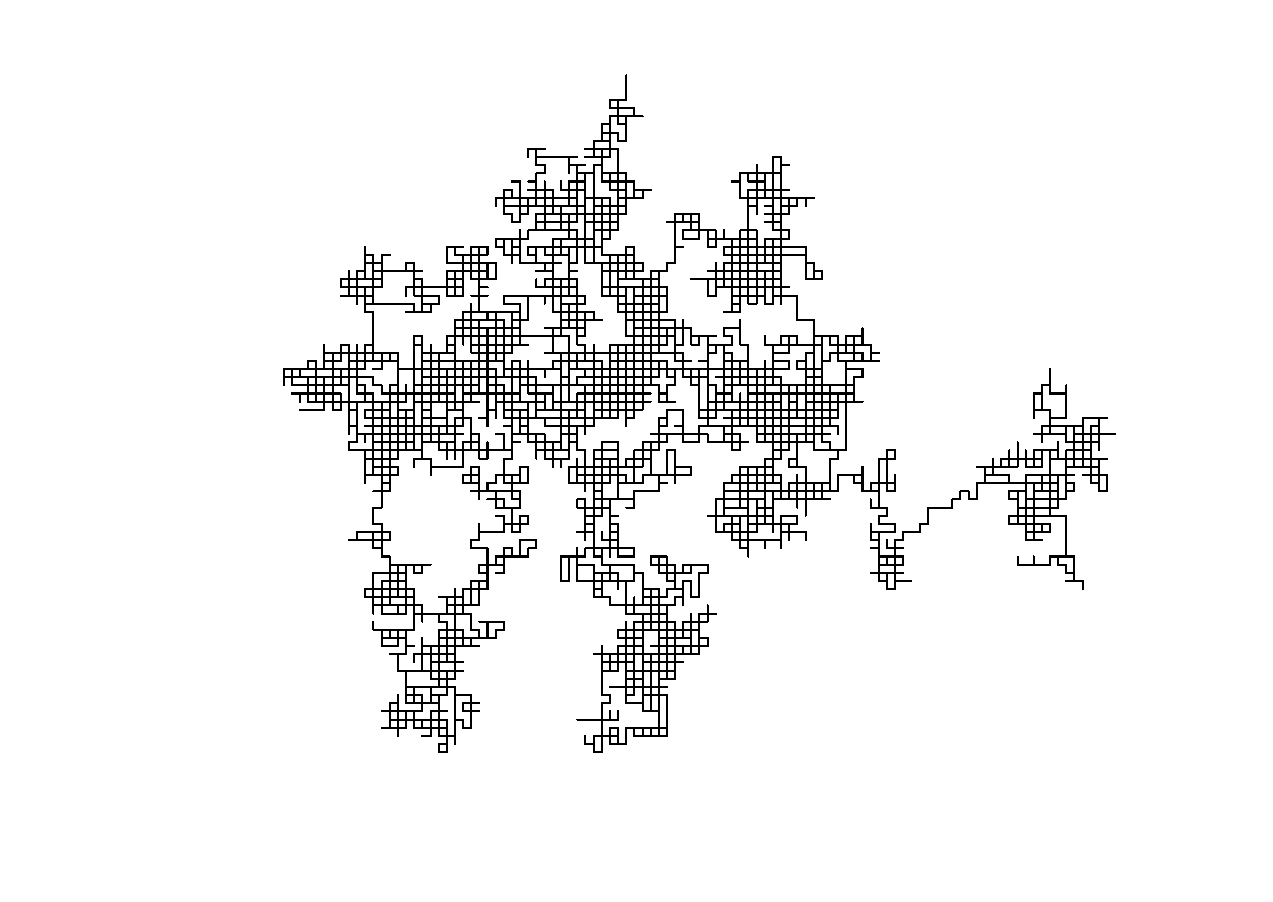
\includegraphics[width=0.5\linewidth]{rwFig}
\caption{Trajectory of a random walk.}\label{fig:rw}
\end{figure}

\subsection*{Monte Carlo Simulation$^{20}$}
Consider the square having vertices $A(1,-1),\: B(1,1),\: C(-1,1),\: D(-1,-1)$ and -- inside this square -- the unit disk.
Choose $n$ random points $P(x,y)$ inside the square, i.e. $-1\le x,y \le 1.$
Let $N$ denote the number of points inside the disk, that is $x^2+y^2\le 1.$
Now, if $n$ is large enough, then
\[\frac{N}{n} \approx \frac{A_{\text{disk}}}{A_{\text{square}}} = \frac{\pi}{4}.\]
Write a program that simulates the above process.
Display the unit disk and the points, also plot the relative frequency: $\frac{N}{n}$ for
all $n=1,2,\dots$ as shown in Figure \ref{fig:mc}.

\begin{figure}[ht!]
\centering
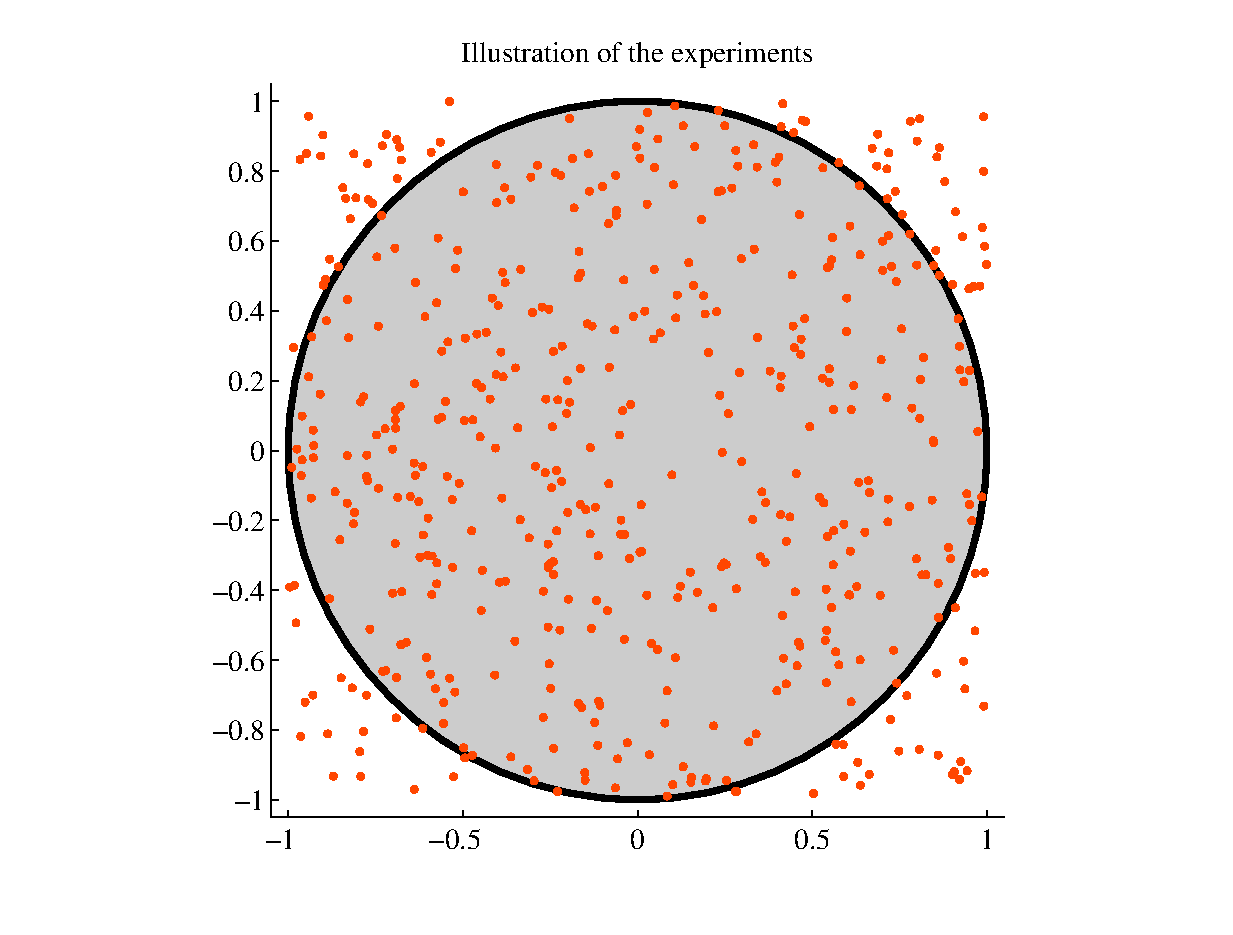
\includegraphics[width=0.48\linewidth]{mcFig1}
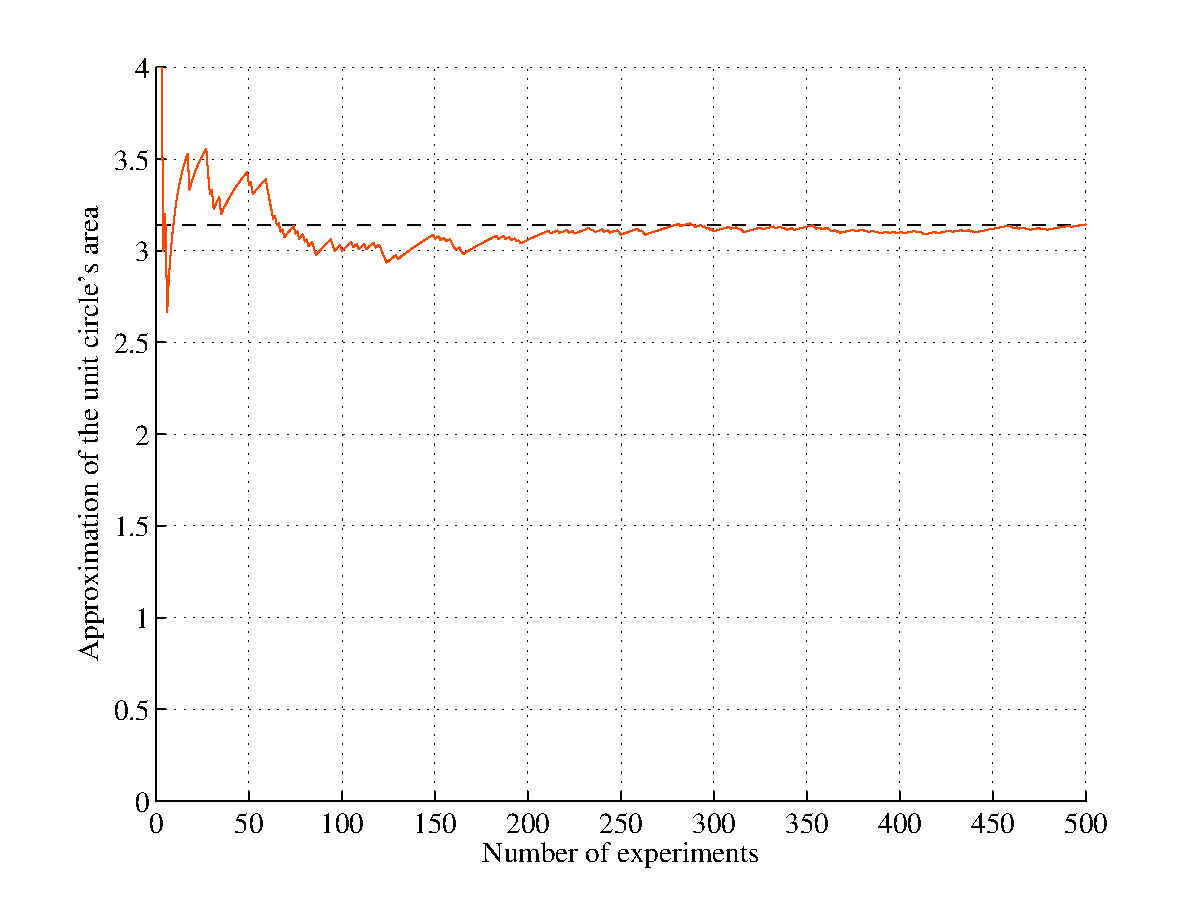
\includegraphics[width=0.48\linewidth]{mcFig2}
\caption{Results of the simulation.}\label{fig:mc}
\end{figure}



\subsection*{Convay's Game of Life$^{30}$}
This game is played on an $n\times n$ grid of 1's and 0's,
where 1 and 0 represent living and dead cells, respectively.
It is clear that every cell has exactly 8 neighbours,
except along the border.
However, we can view these border cells, as if they had 8 neighbours,
considering the cells outside the border dead.
The population of cells advances to a new generation by
applying the following rules for every cell (from Wikipedia):
\begin{itemize}
 \item Any live cell with fewer than two live neighbours dies, as if caused by under-population.
 \item Any live cell with two or three live neighbours lives on to the next generation.
 \item Any live cell with more than three live neighbours dies, as if by overcrowding.
 \item Any dead cell with exactly three live neighbours becomes a live cell, as if by reproduction.
\end{itemize}

Write a program that for a given table, computes the next generation.
For example:
\[
\begin{bmatrix}
 0 & 1 & 1 & 0\\
 1 & 1 & 0 & 1\\
 0 & 1 & 1 & 1\\
 1 & 0 & 1 & 1
\end{bmatrix}
\quad \longrightarrow
\quad
\begin{bmatrix}
 1 & 1 & 1 & 0\\
 1 & 0 & 0 & 1\\
 0 & 0 & 0 & 0\\
 0 & 0 & 0 & 1
\end{bmatrix}
\]
Look up the \mc{image} object in the documentation, and
use it to display the original and new generation in separate figures.

\subsection*{PageRank$^{30}$}
This algorithm was first used by Google to order search results.
According to Google:
\begin{quote}
PageRank works by counting the number and quality of links to a page to determine a rough estimate of how important the website is.
The underlying assumption is that more important websites are likely to receive more links from other websites.
\end{quote}
From this perspective the internet consists of webpages and links between them (see Figure \ref{fig:graph}).
\begin{figure}[ht!]
 \centering
 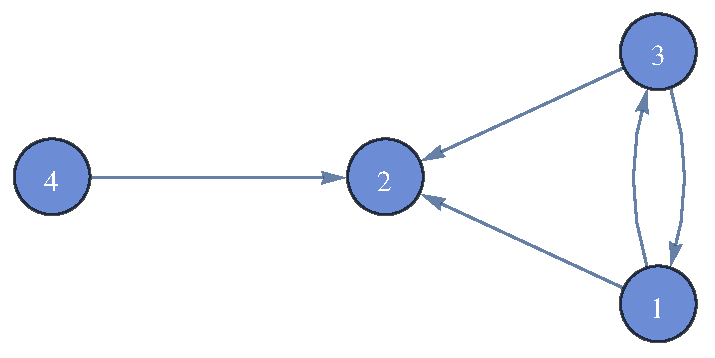
\includegraphics[width=0.5\textwidth]{graph}
 \caption{An example graph with $n=4$ edges.}\label{fig:graph}
\end{figure}
The graph in Figure~\ref{fig:graph} is represented as two arrays: vertecies ($V$) and edges ($E$)
in the following way:
\[V=
\begin{bmatrix}
1 & 2 & 3 & 4
\end{bmatrix},
\quad
E=\begin{bmatrix}
1 & 1 & 3 & 3 & 4\\
2 & 3 & 1 & 2 & 2
\end{bmatrix}.
\]
Denote the number of vertices by $n,$ which is $n=4$ in our example.
Now we construct the adjacency matrix $A$ of the graph, that is we have $A_{ij}=1$
if and only if the graph has the edge $i\to j,$ otherwise $A_{ij}=0.$
It could be that, some of the rows have only zero entries, which are quite problematic, therefore
we need to substitute every such row with a row full of ones to get a new matrix $B.$
This means, that if we have webpages that don't link to anywere, than we assume
instead they link to everywhere.
For the example graph, they look like this:
\[
A = 
\begin{bmatrix}
0 & 1 & 1 & 0\\
0 & 0 & 0 & 0\\
1 & 1 & 0 & 0\\
0 & 1 & 0 & 0
\end{bmatrix}
\qquad\longrightarrow
\qquad
B = 
\begin{bmatrix}
0 & 1 & 1 & 0\\
1 & 1 & 1 & 1\\
1 & 1 & 0 & 0\\
0 & 1 & 0 & 0
\end{bmatrix}.
\]
The next step is to make sure that every row sums up to one, thus we need to normalize the rows of $B$
by which we obtain the matrix $M$ with entries
\[M_{ij} := \frac{B_{ij}}{\sum_{k=1}^n B_{ik}} = \frac{B_{ij}}{B_{i1} + B_{i2} + \dots + B_{in}}.\]
Continuing the example, we have:
\[
M = 
\begin{bmatrix}
0 & \frac{1}{2} & \frac{1}{2} & 0\\
\frac{1}{4} & \frac{1}{4} & \frac{1}{4} & \frac{1}{4}\\
\frac{1}{2} & \frac{1}{2} & 0 & 0\\
0 & 1 & 0 & 0
\end{bmatrix}.
\]
In order to regularize the problem, we need to perturb the matrix $M$ with the matrix $S,$
that is \[P:=\alpha M + (1-\alpha)S,\]
where  $S_{ij} := 1/n.$
Following Google's recommendation we set $\alpha := 0.8.$ The example becomes:
\[P = \frac{4}{5}\begin{bmatrix}
0 & \frac{1}{2} & \frac{1}{2} & 0\\
\frac{1}{4} & \frac{1}{4} & \frac{1}{4} & \frac{1}{4}\\
\frac{1}{2} & \frac{1}{2} & 0 & 0\\
0 & 1 & 0 & 0
\end{bmatrix} + \frac{1}{5} 
\begin{bmatrix}
\frac{1}{4} & \frac{1}{4} & \frac{1}{4} & \frac{1}{4}\\
\frac{1}{4} & \frac{1}{4} & \frac{1}{4} & \frac{1}{4}\\
\frac{1}{4} & \frac{1}{4} & \frac{1}{4} & \frac{1}{4}\\
\frac{1}{4} & \frac{1}{4} & \frac{1}{4} & \frac{1}{4}
\end{bmatrix}=
\frac{1}{20}
\begin{bmatrix}
1 & 9 & 9 & 1\\
5 & 5 & 5 & 5\\
9 & 9 & 1 & 1\\
1 & 17 & 1 & 1
\end{bmatrix}
\]
Now, in the last step we need to solve the linear equation $P^\top x=x$ for the unkown vector $x.$
This $x$ vector will contain the ranking scores for each webpage.
The equation $P^\top x=x$ is equivalent to the homogeneous equation $(P^\top-I)x=0,$
where $I$ is the $n\times n$ identity matrix.
Due to the earlier regularization, we can be sure there is only one
$x$ vector satisfying this equation\footnote{It is clear that both $x$ and let's say $1.34\cdot x$
imply the same ranking.
So actually, there are infinitely many solutions for $P^\top x = x,$
but they only differ in a scalar factor, thus implying the same ranking.}.
Finally, normalize the result, so that the ranking scores sum up to 1:
\[r := \frac{x}{\sum_{i=1}^n x_i}.\]
The ranking scores for the example: $r = [0.223,\: 0.426,\: 0.223,\: 0.128],$
so the ranking is $R = [2,\: 3,\: 1,\: 4].$

Write a program that for a given $V$ and $E$ computes the ranking.
Use randomly generated test graphs to test your program.
Make sure that the test graph is a simple (directed) graph, i.e. it does not contain
loops or multiple edges.






\chapter{Data Types, Functions and Flow Control}
\section{Exercises}
\begin{prb*}{3}
Create a structure array named {\tt subject} with the following fields: {\tt .name}, {\tt.age}, {\tt.weight}, {\tt.height}
using data from Table~\ref{tab:sub}, and determine the
\begin{multicols}{2}
 \begin{enumerate}[a)]
  \item average age
  \item mean and standard deviation of the weights 
  \item names of the 3 oldest subjects
  \item names of those who are younger than $25$
  \item average age of those who are taller than 160\,cm, and not heavier than 60\,kg
  \item names of those who have height above average
 \end{enumerate}
\end{multicols}
\begin{table}[ht!]
 \centering
 \begin{tabular}{lccc}
  \toprule
  \multicolumn{4}{c}{Subject}\\
  \midrule
  Name & Age & Weight & Height\\
  \midrule
  Judy Garcia  	  & 23 & 59 & 167\\
  Robert Baker 	  & 22 & 66 & 180\\
  Laura Ross 	  & 28 & 70 & 171\\
  Kimberly Price  & 21 & 45 & 162\\
  Nancy Thompson  & 27 & 90 & 165\\
  Tina Clark 	  & 28 & 77 & 191\\
  \bottomrule
 \end{tabular}
 \caption{Data for creating the structure {\tt subject}.}\label{tab:sub}
\end{table}
\end{prb*}

\begin{prb*}{5}
 Write a script that you can use to manage the structure {\tt subject}.
 At the start it should be checked (\mc{exist}) whether there is a variable in the Work Space called {\tt subject}
 or not, in the latter case it should be checked if there is a file {\tt subject.m}, and then loaded (\mc{load}) into the Work Space.
 If neither the variable nor the file exist; an empty structure should be initialized. 
 Create a menu for your program with the following items:
 \begin{description}
  \item[New] Create new entry in {\tt subject}. The program should ask for the subject's name, age, weight and height. 
  \item[View] Print out the name of every subject.
  \item[Exit] Before quitting, the program should ask whether to save the changes or not, and act accordingly (\mc{save}). 
 \end{description}
\end{prb*}




\begin{prb*}{5}
Write a function that, for a given subject,
calculates the body mass index.
Specifically, write a function named \mc{get\_bmi} with one input and three (optional) outputs:
\begin{description}
 \item[\mc{get\_bmi}\mck{(s)}] prints out the name and textual classification of the subject {\tt s},
 \item[\mck{bmi = }\mc{get\_bmi}\mck{(s)}] gives the body mass index of subject {\tt s},
 \item[\mck{[bmi, bmi\_class] = }\mc{get\_bmi}\mck{(s)}] gives the body mass index and numeric classification. 
\end{description}

\begin{table}[ht!]
 \centering
 \begin{tabular}{clc}
  \toprule
  & \multicolumn{2}{c}{Classification}\\
  \cmidrule(r){2-3}
  BMI [$\mathrm{kg}/\mathrm{m}^2$] & Text & Number \\
  \midrule
  --15 	 & very severely underweight 	& $-3$\\
  15--16 & severely underweight 	& $-2$\\
  16--18.5 & underweight 		& $-1$\\
  \midrule
  18.5--25 & normal 			& $0$\\
  \midrule
  25--30   & overweight			& $1$\\
  30--35   & moderately obese 		& $2$\\
  35--   & severely obese 		& $3$\\
  \bottomrule
 \end{tabular}\label{tab:BMI}
 \caption{BMI classification}
\end{table}
\end{prb*}

\begin{prb*}{2}
Using the following cells
\begin{center}
\mck{ranks =  \{2,3,4,5,6,7,8,10,J,Q,K,A\}},\quad \mck{suits =  \{Clubs,Diamonds,Hearts,Spades\}}
\end{center}
create the standard 52-card deck as a cell containing all pairs: \mck{\{\{'2','Clubs'\}, \{'3','Clubs'\},\dots\}}. 
\end{prb*}


\begin{prb*}{2}
Determine how many different ways the number $1729$ can be decomposed to a sum of two cubes of positive integers, i.e. integers $a,b>0$ satisfying $a^3 + b^3 = 1729.$
Use trial and error for all integers $1\le a\le b\le 12.$
\end{prb*}


\begin{prb*}{2}
Using trial and error, determine the Pythagorean triples: $a^2 + b^2 = c^2$ for all $1\le a\le b\le c\le 100$.
\end{prb*}

\begin{prb*}{5}
Let $M$ a natural number, and consider the (finite) sequence $u(M)=\begin{bmatrix}u_0 & u_1 & \dots & u_n\end{bmatrix}^\top$
generated by a given function $f\colon \N\to \N$ in the following way:
\[u(M) = \begin{bmatrix}
          M& f(M)&\ f(f(M)) & f^3(M) & \dots & f^n(M)
         \end{bmatrix}\quad \text{or equivalently} \quad u_0:=M,\ u_{k+1} = f(u_k),\]
where 
\[f(n) = \begin{cases}
            n/2, & \text{if }n \text{ is even,}\\
            3n+1 & \text{if }n \text{ is odd,}
           \end{cases}
\]
The famous Collatz conjecture states that starting from any natural number $M$ the sequence $u(M)$ will eventually
reach $1.$
Assuming the conjecture is true, let $n$ the smallest number such that $f^n(M) = 1,$
so that the last element in the list $u(M)$ is $u_n=1.$ 
The number of steps taken to reach 1 is called stopping time $T(M)$.
For example:
\[u(17)=[17, 52, 26, 13, 40, 20, 10, 5, 16, 8, 4, 2, 1], \quad T(17) = 12.\]
Write a function named \mck{u = }\mc{collatz}\mck{(M)}.
Plot $(M,\max u(M)).$ Plot the histogram of the stopping time $T(M)$ for $2\le M \le 500.$
\end{prb*}

\begin{prb*}{4}
Implement the quicksort algorithm as a function \mck{v = }\mc{quicksort}\mck{(u)}, where
$u,\,v$ are lists, and $v$ is the sorted version of $u.$
\begin{quote}
The quicksort algorithm (from Wikipedia):
\begin{enumerate}
 \item Pick an element, called a pivot, from the array.
 \item Reorder the array so that all elements with values less than the pivot come before the pivot, while all elements with values greater than the pivot come after it (equal values can go either way). After this partitioning, the pivot is in its final position. This is called the partition operation.
 \item Recursively apply the above steps to the sub-array of elements with smaller values and separately to the sub-array of elements with greater values.
\end{enumerate}


\end{quote}

\end{prb*}


\section{Projects}
\subsection*{Simple Game$^{30}$}
In this game the computer thinks of a number $ 1\le n\le 100$, then you have to guess that number.
Each time you guess, the computer tells you whether your guess is too small or too large.
As soon as you guess the correct number the game is over.
Every time the game is played the time (score) that was needed to find the number should be recorded.

To store information about the players and their scores use the structure \mck{game} with fields:
\begin{description}
 \item[\mck{.player}] A structure array with fields:
  \begin{description}
  \item[\mck{.name}] A string, the name of the player.
  \item[\mck{.time}] A vector containing the player's scores. Should be an empty vector, if no game has been played yet.
 \end{description}
 \item[\mck{.cp}] An integer representing the current player, such that \mck{game.player(game.cp)} refers to the
		  structure corresponding to the current player.
\end{description}
Make sure, that the variable \mck{game} exists in the Work Space by
loading a previously saved one, or -- if the file does not exist then -- initializing one (with at least one player). 

Create a menu for the game with the following items:
\begin{description}
\item[Start] 
    Starts the game by calling the function \mc{start\_game}.
    Write a function named \mck{game\_new =}\mc{ start\_game}\mck{(game)}, so that -- after finishing the game --
    it appends the time (needed to succed) to the current player's time vector; and returns with the updated structure \mck{game\_new}.
\item[Change Player]
    Change the current player by calling the function \mc{change\_player}.
    Write a function named \mck{game\_new = }\mc{change\_player}\mck{(game)} that
    lists all players, from which the user can choose one; and returns with the structure \mck{game\_new}
    where the current player (\mck{game.cp}) has been updated -- in accordance with the user's choice.
\item[New Player]
    Add a new player by calling the function \mc{new\_player}. Write a function named \mck{game\_new = }\mc{new\_player}\mck{(game)} that adds a new entry to the structure array \mck{game.player} by asking the player's name,
    and returning with the updated structure \mck{game\_new}.
    The new player's  time vector should be empty. When a new player is added, make sure that the the current player is set to the new player.
\item[View Ranking]
    List the top 5 players and their scores by calling the function \mc{view\_ranking}.
\item[Quit]
    Quit the program. Save the variable \mck{game} using \mc{save}.
\end{description}
Make sure that besides the menu the current player's name is also displayed.

\subsection*{Euler Solver$^{30}$}
Differential equations play a central role in modeling dynamical systems, such as the weather,
the chemical processes in a cell or the motion of a commet.
Henceforth, we only consider deterministic continuous models that can be described by
an explicit, first order ordinary differential equation in the form:
\begin{equation}
\dot x(t) = f(t,x(t)),\quad x(t_0) = x_0,\label{eq:ode} 
\end{equation}
for some interval $t\in [t_0, t_N],$
where $x\colon \R\to\R^n$ the state variable, and $f\colon\R\times\R^n\to\R^n$ is the model.
In general, we can only calculate the approximate solution of \eqref{eq:ode} in discrete points $t_1,t_2,\dots,t_N.$
The solution at these points are approximated $x(t_n)\approx x_n$ by using the forward Euler method:
\[t_{n+1} = t_n + h, \quad x_{n+1} = x_n + h f(t_n, x_n), \qquad n=0,1,\dots,N-1\]
where $h$ is the step size, a fixed small positive number.

Write a function named \mck{sol = }\mc{euler\_solve}\mck{(ivp)}
where the input \mck{ivp} is a structure defining the initial value problem \eqref{eq:ode},
having the following fields:
\begin{description}
 \item[\mck{.model}] is a function handle for the function $f\colon \R\times\R^n\to\R^n,$
 \item[\mck{.initial\_value}] is the initial vector $x_0\in\R^n,$
 \item[\mck{.interval}] is an array \mck{[t0, tN]}, where $t_0$ and $t_N$ are the initial and final time, respectively.
 \item[\mck{.step\_size}] is the step size $h,$ if it's empty use $h:=|t_N-t_0|\cdot 10^{-3}.$
\end{description}
The output \mck{sol} is a structure with fields \mck{.t} which contains the time vector $[t_0,t_0+h,\dots,t_0+Nh],$
and \mck{.x} which contains the approximation of the solutions $x_1(t),\,x_2(t),\dots,x_n(t)$ in its rows.

Test your solver by writing scripts for the following problems:
\begin{enumerate}[a)]
\item Solve the logistic equation: $\dot x = x(1-x)$ for the initial values $x(0):=x_0\in\{0,0.25,0.5,\dots,2\},$
      and plot the solutions (see Figure \ref{fig:logistic}).
\item Solve the equation $\ddot u + 2\xi\dot u + u = 0$ of a damped oscillator -- with the initial value
$u(0) := 1,\: \dot u(0) := 0$ -- for the damping parameters $\xi =0.2,0.3,\dots,1.4,$
      and plot the solutions (see Figure \ref{fig:damped}).\\
      {\it \small Hint: to write the oscillator in the form of \eqref{eq:ode} set $x=(x_1\ \ x_2)^\top:=(u\ \ \dot u)^\top.$}
      \begin{figure}[ht!]
	\centering
	\begin{subfigure}[b]{0.48\textwidth}
	  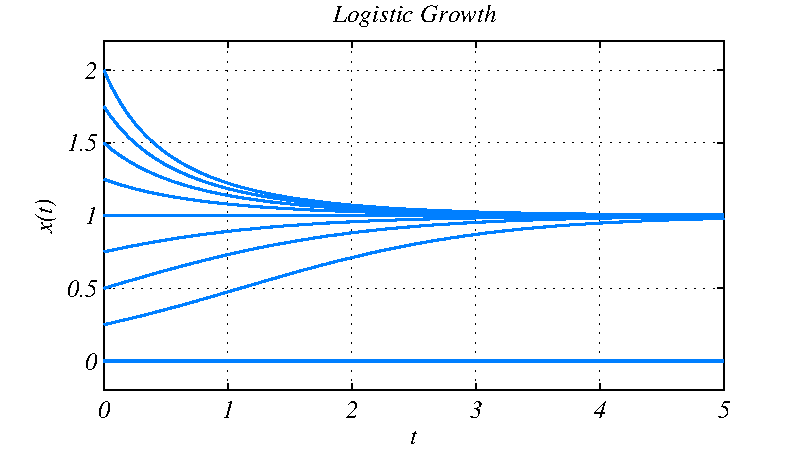
\includegraphics[width=\textwidth]{logistic}
	  \caption{Logistic equation for different initial values.}
	  \label{fig:logistic}
	\end{subfigure}
	\begin{subfigure}[b]{0.48\textwidth}
	 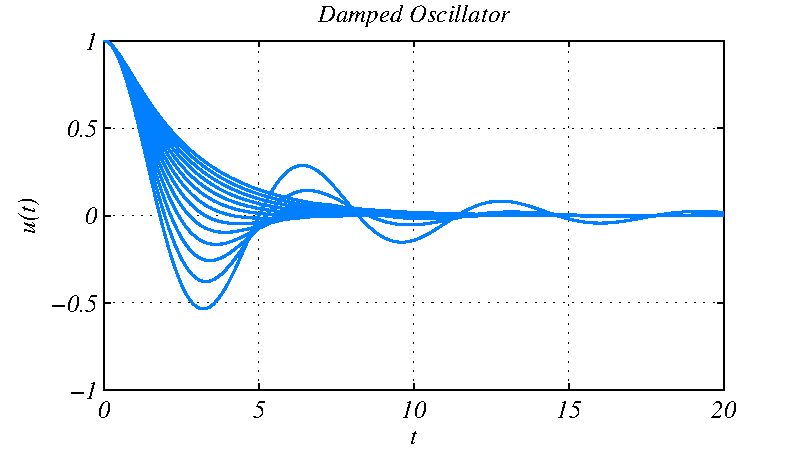
\includegraphics[width=\textwidth]{damped}
	 \caption{Damped oscillator for different dampings.}
	  \label{fig:damped}
	\end{subfigure}
	\caption{Solutions of the logistic equation and the damped oscillator.}
      \end{figure}

\item Solve the Lorenz system:
	\begin{equation}
	    \dot u = 10(v-u),\qquad
	    \dot v = u(28-w)-v,\qquad
	    \dot w = uv - \frac{8}{3}z,\label{eq:lorenz}
	\end{equation}
	\begin{figure}[ht!]
	\centering
	 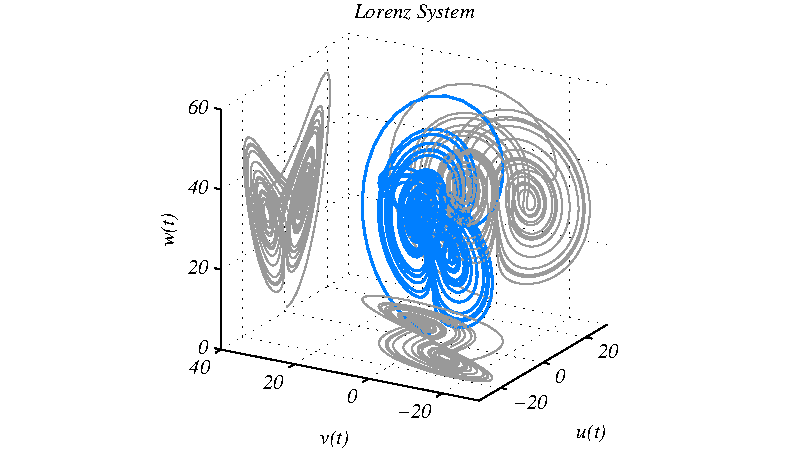
\includegraphics[width=0.8\textwidth]{lorenz}
	 \caption{A trajectory and its projections of the Lorenz System.}\label{fig:lorenz}
	\end{figure}

      for the initial value $x(0) = (u(0)\ v(0)\ w(0))^\top := (1\ 1\ 1)^\top,$
      and plot the  trajectory $t\mapsto (u(t), v(t), w(t))$ in three dimensions using \mc{plot3} (see Figure~\ref{fig:lorenz}).
      Show the following projections of the trajectory as well: $t\mapsto (30, v(t), w(t)),\: t\mapsto (u(t), 30, w(t)),\: t\mapsto (u(t), v(t), 0).$
\end{enumerate}

\subsection*{Cellular Automaton$^{30}$}
Let $x_1=[x_{1,1},x_{1,2},\dots,x_{1,m}]$ a list of zeros and ones representing the state of the automaton.
At each step the state of automaton evolves by a set of rules.
For a given rule $r$ the state is updated by
\[x_{i+1,k} = f_r(x_{i,k-1}, x_{i,k}, x_{i,k+1}),\quad k=1,2,\dots,m\]
with the assumption $x_{i,0} = x_{i,m+1} = 0$ for all $i=1,2,\dots,n.$
\begin{table}[ht!]\centering
 \begin{tabular}{ccccccccccccc}
 \toprule
      &     &     &  &\multicolumn{8}{c}{rules} \\
      \cmidrule{5-13}
  $a$ & $b$ & $c$ &  & 0 & 1 & 2 & 3 & 4 &\dots & 30 &\dots  & 255 \\
  \midrule
%  & & & & \multicolumn{5}{c}{$f_r(u_{k-1},u_k,u_{k+1})$} \\
  0 & 0 & 0 & $d_0(r)$ & 0 & 1 & 0 & 1 & 0 & \dots & 0 &\dots & 1\\
  0 & 0 & 1 & $d_1(r)$ & 0 & 0 & 1 & 1 & 0 & \dots & 1 &\dots & 1\\
  0 & 1 & 0 & $d_2(r)$ & 0 & 0 & 0 & 0 & 1 & \dots & 1 &\dots & 1\\
  0 & 1 & 1 & $d_3(r)$ & 0 & 0 & 0 & 0 & 0 & \dots & 1 &\dots & 1\\
  1 & 0 & 0 & $d_4(r)$ & 0 & 0 & 0 & 0 & 0 & \dots & 1 &\dots & 1\\
  1 & 0 & 1 & $d_5(r)$ & 0 & 0 & 0 & 0 & 0 & \dots & 0 &\dots & 1\\
  1 & 1 & 0 & $d_6(r)$ & 0 & 0 & 0 & 0 & 0 & \dots & 0 &\dots & 1\\
  1 & 1 & 1 & $d_7(r)$ & 0 & 0 & 0 & 0 & 0 & \dots & 0 &\dots & 1\\
  \bottomrule
 \end{tabular}
\caption{All possible rules. Columns $0,1,2,\dots$ contain the digits of the corresponding rule in base 2.}\label{tab:rules}
\end{table}
Any rule $r=0,1,2,\dots,255$ in base 2 has at most 8 digits, and can be written as
\[r = d_0(r) + 2 d_1(r) + 2^2d_2(r) + \dots + 2^7d_7(r), \qquad d_i(r)\in\{0,1\},\quad i=0,2,\dots,7.\]
The map $f_r$ is defined as $f_r(a,b,c) = d_i(r),$ where $i=2^2a + 2b + c.$
For instance, consider $r = 30 = 2^1 + 2^2 + 2^3 + 2^4,$ so $d_0(30) = 0,\: d_1(30) = 1,\: d_2(30) = 1,$ etc.
Therefore $f_{30}(0,0,0)=d_0(30) = 0,\: f_{30}(0,0,1)=d_1(30) = 1,\: f_{30}(0,1,0)=d_2(30) = 1,$ etc., for summary see Table~\ref{tab:rules}.
\begin{figure}[ht!]
\centering
  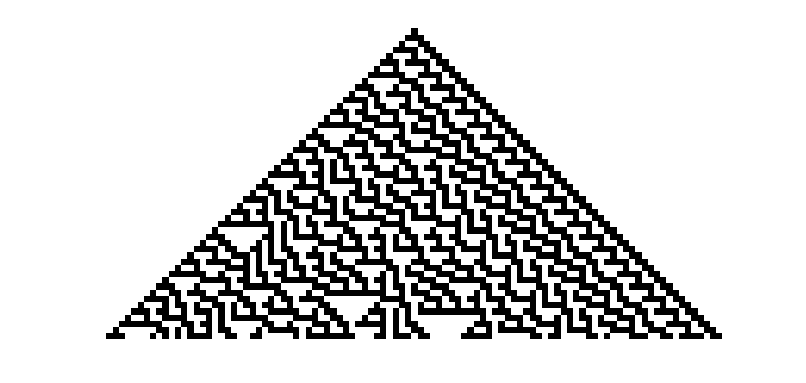
\includegraphics[width=0.7\textwidth]{rule30}
  \caption{Rule 30, generated using \mc{cellular\_automaton}\mck{(30,\,[50,\,100],\,50)}.}\label{fig:automaton}
\end{figure}

The evolution of an initial state $x_1=[x_{1,1},x_{1,2},\dots,x_{1,m}]$ for $n$ steps is collected in the matrix
\[X = \begin{bmatrix}
       x_1\\
       x_2\\
       \vdots\\
       x_n
      \end{bmatrix} = 
     \begin{bmatrix}
       x_{1,1} & x_{1,2} & \dots & x_{1,m}\\
       x_{2,1} & x_{2,2} & \dots & x_{2,m}\\
       \vdots & \vdots & \ddots & \vdots\\
       x_{n,1} & x_{n,2} & \dots & x_{n,m}
      \end{bmatrix}.
      \]
Write a function named \mc{cellular\_automaton} considering the following specification:
\begin{description}
  \item[\mc{cellular\_automaton}\mck{(r, [n,\,m])}] shows the evolution of the initial state $x_1$  as an image by the rule $r$ for $n$ steps, where the initial state is $x_{1,1}=1,$ $x_{1,i}=0$ for all $i=2,\dots,m.$
  \item[\mc{cellular\_automaton}\mck{(r, n)}] is the same as before except $m=n.$
  \item[\mc{cellular\_automaton}\mck{(r, [n,\, m], [i1,\,i2\,\dots,\,ik])}] is the same as before except the initial state is defined by $x_{1,i}=1$ for all $i\in\{i_1,i_2,\dots,i_k\}$ and $x_{1,i}=0$ otherwise. See an example in Figure \ref{fig:automaton}.
  \item[\mck{X = }\mc{cellular\_automaton}\mck{(r, \dots)}] instead of plotting, it returns with a matrix $X$ containing the states of the automaton as its rows.
\end{description}

\subsection*{Iterated Function System$^{30}$}
Given a polygon $S$ in the plane represented by its $m$ vertices $u_{i}=(x_i\ y_i)^\top,$ and a set of of affine contraction maps:
\[S =  \begin{bmatrix}
	    u_{1}\\
	    u_{2}\\
	    \vdots\\
	    u_{m}
        \end{bmatrix},\qquad F_i(u):=A_i u + b_i, \quad A_i\in\R^{2\times 2},\,b_i\in\R^2, \quad i=1,2,\dots,n.\]
One can apply $F_i$ to the polygon $S$ and get an other polygon $F_i(S)$ by applying $F_i$
to every vertices of the polygon in the following way:
\[F_i(S) = 
	    \begin{bmatrix}
	      F_i(u_{1})\\
	      F_i(u_{2})\\
	      \vdots\\
	      F_i(u_{m})\\
	    \end{bmatrix}=
	    \begin{bmatrix}
	      A_iu_{1}+b_i\\
	      A_iu_{2}+b_i\\
	      \vdots\\
	      A_iu_{m}+b_i\\
	    \end{bmatrix}.
\]
Generate new polygons recursively by
\[X_{k+1} = \begin{bmatrix}
             F_1(X_k) & F_2(X_k) & \dots\ & F_n(X_k)
            \end{bmatrix}
, \qquad X_0 = S,\]
where $X_k$ is a matrix containing polygons as its columns, and $F_i(X_k)$ means that $F_i$
applied column-wise, that is applied to every polygon contained in $X_k.$

For example, when the polygons are triangles $m=3$, and we have two transformations $F_1,\,F_2$ so that $n=2.$ 
\[
X_0 =\begin{bmatrix}
      u_{1}\\
      u_{2}\\
      u_{3}
     \end{bmatrix},\quad
X_1 =\begin{bmatrix}
      F_1(X_0) & F_2(X_0)
     \end{bmatrix},\quad
\]
\[
X_2 =\begin{bmatrix}
      F_1(X_1) & F_2(X_1))
     \end{bmatrix}=
     \begin{bmatrix}
      F_1(F_1(X_0)) & F_1(F_2(X_0)) & F_2(F_1(X_0)) & F_2(F_2(X_0))
     \end{bmatrix}.
\]

Write a function named \mc{ifs} considering the following specification:
\begin{description}
 \item[\mc{ifs}\mck{(ifs\_data)}] shows the polygons determined by the input (see below the input specification).
 \item[\mck{X = }\mc{ifs}\mck{(ifs\_data)}] instead of plotting it gives the matrix $X_k.$
 \item[\mc{ifs}\mck{(ifs\_data, 'Color', [1,0,0], \dots)}] excepts extra arguments as an option for \mc{patch} object.
\end{description}

The input structure \mck{ifs\_data} has the following fields:
\begin{description}
 \item[\mck{.initial\_shape}] a vector representing the initial polygon $S.$
 \item[\mck{.transformation}] a cell containing the matrices $A_i,\ i=1,2\dots,n$
 \item[\mck{.dilation}] a cell containing the dilations $b_i,\ i=1,2\dots,n$
 \item[\mck{.step}] is an integer $N,$ then the iteration goes $N$ steps, thus calculating $X_N.$
		    Note that the size of $X_N$ is $2m\times n^N.$
\end{description}

Test your function by writing a script for the following problems:
\begin{enumerate}[a)]
 \item Show the 6th approximation of the Sierpinski triangle:
 \[A_1 = A_2 = A_3 = \begin{bmatrix}
          1/2 & 0\\
          0   & 1/2
         \end{bmatrix},\quad
         b_1 = \begin{bmatrix}
          0 \\
          0  
         \end{bmatrix},\quad
         b_2 = \begin{bmatrix}
          1/2 \\
          0  
         \end{bmatrix},\quad
         b_3 = \begin{bmatrix}
          1/4 \\
          \sqrt{3}/4
         \end{bmatrix},
\]
starting from the equilateral triangle: $S=\begin{bmatrix}0 & 0 & 1 & 0 & 1/2 & \sqrt{3}/2\end{bmatrix}^\top.$
The Figure \ref{fig:ifs}. shows the first three approximation of the Sierpinski triangle.
Try out what happens when you start from the square: $S=\begin{bmatrix}0 & 0 & 1 & 0 & 1 & 1 & 0 & 1\end{bmatrix}^\top.$
\begin{figure}[ht!]
\centering
  
\includegraphics[width=0.3\textwidth]{ifs1}
  
\includegraphics[width=0.3\textwidth]{ifs2}
  
\includegraphics[width=0.3\textwidth]{ifs3}
  \caption{Approximations of the the Sierpinski triangle: $X_0,\,X_1,\,X_2$.}\label{fig:ifs}
\end{figure}
\item Show the 4th approximation of the Sierpinski carpet:
 \[A_1 =  \dots = A_8 = \begin{bmatrix}
          1/3 & 0\\
          0   & 1/3
         \end{bmatrix}\]
\[       b_1 = \begin{bmatrix}
          0 \\
          0  
         \end{bmatrix},\
         b_2 = \begin{bmatrix}
          1 \\
          0  
         \end{bmatrix},\
         b_3 = \begin{bmatrix}
          2 \\
          0
         \end{bmatrix},\
         b_4 = \begin{bmatrix}
          0 \\
          1
         \end{bmatrix},\
         b_5 = \begin{bmatrix}
          2 \\
          1
         \end{bmatrix},\
         b_6 = \begin{bmatrix}
          0 \\
          2
         \end{bmatrix},\
         b_7 = \begin{bmatrix}
          1 \\
          2
         \end{bmatrix},\
         b_8 = \begin{bmatrix}
          2 \\
          2
         \end{bmatrix},
\]
starting from the square: $S=\begin{bmatrix}0 & 0 & 3 & 0 & 3 & 3 & 0 & 3\end{bmatrix}^\top.$
\begin{figure}[ht!]
\centering
  
\includegraphics[width=0.3\textwidth]{carpet1}
  
\includegraphics[width=0.3\textwidth]{carpet2}
  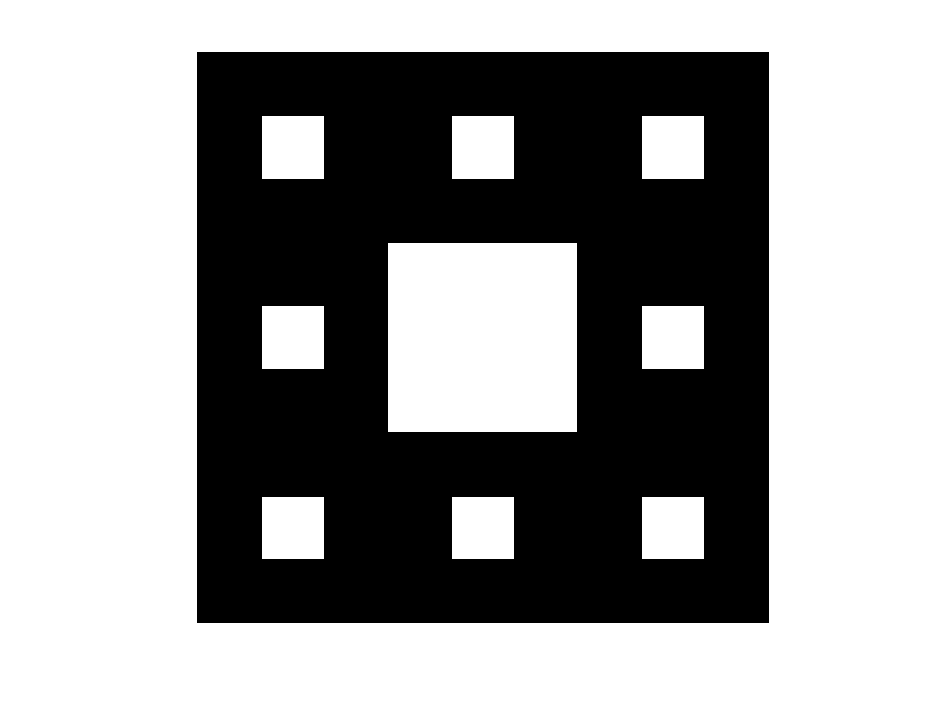
\includegraphics[width=0.3\textwidth]{carpet3}
  \caption{Approximations of the Sierpinski triangle: $X_0,\,X_1,\,X_2$.}\label{fig:ifs}
\end{figure}
\item Show the 9th approximation of the Dragon curve:
\[
A_1 = \frac{1}{\sqrt{2}}\begin{bmatrix}
          \cos(\pi/4) & \sin(\pi/4)\\
          -\sin(\pi/4) & \cos(\pi/4)
         \end{bmatrix},\quad
A_2 = \frac{1}{\sqrt{2}}\begin{bmatrix}
          \cos(5\pi/4) & -\sin(5\pi/4)\\
          \sin(5\pi/4) & \cos(5\pi/4)
         \end{bmatrix}
\]
\[       b_1 = \begin{bmatrix}
          0 \\
          0  
         \end{bmatrix},\
         b_2 = \begin{bmatrix}
          1 \\
          0  
         \end{bmatrix}
\]
in blue (see Figure \ref{fig:dragon}.), starting from the initial polygon $S= \begin{bmatrix}0 & -0.05 & 1 & -0.05 & 1 & 0.05 & 0 & 0.05\end{bmatrix}^\top.$
\begin{figure}[ht!]
\centering
  
\includegraphics[width=0.3\textwidth]{dragon1}
  
\includegraphics[width=0.3\textwidth]{dragon2}
  
\includegraphics[width=0.3\textwidth]{dragon3}
  \caption{Approximations of the dragon curve: $X_0,\ X_1,\ X_2$.}\label{fig:dragon}
\end{figure}
\end{enumerate}

\end{document}



\[S_1 = \begin{bmatrix}
	    F_1(u_{1,1}) & F_2(u_1) & \dots & F_n(u_1)\\
	    F_1(u_{2,1}) & F_2(u_2) & \dots & F_n(u_2)\\
	    \vdots\\
	    F_1(u_{m,1}) & F_2(u_m) & \dots & F_n(u_m)\\
        \end{bmatrix}
\]